% !TEX TS-program = pdflatex
% !TEX encoding = UTF-8 Unicode

% This is a simple template for a LaTeX document using the "article" class.
% See "book", "report", "letter" for other types of document.

\documentclass[11pt]{article} % use larger type; default would be 10pt

\usepackage[utf8]{inputenc} % set input encoding (not needed with XeLaTeX)

%%% Examples of Article customizations
% These packages are optional, depending whether you want the features they provide.
% See the LaTeX Companion or other references for full information.

%%% PAGE DIMENSIONS
\usepackage{geometry} % to change the page dimensions
\geometry{a4paper} % or letterpaper (US) or a5paper or....
% \geometry{margin=2in} % for example, change the margins to 2 inches all round
% \geometry{landscape} % set up the page for landscape
%   read geometry.pdf for detailed page layout information

\usepackage{graphicx} % support the \includegraphics command and options

% \usepackage[parfill]{parskip} % Activate to begin paragraphs with an empty line rather than an indent

%%% PACKAGES
\usepackage{booktabs} % for much better looking tables
\usepackage{array} % for better arrays (eg matrices) in maths
\usepackage{paralist} % very flexible & customisable lists (eg. enumerate/itemize, etc.)
\usepackage{verbatim} % adds environment for commenting out blocks of text & for better verbatim
\usepackage{subfig} % make it possible to include more than one captioned figure/table in a single float
\usepackage{graphicx}
% These packages are all incorporated in the memoir class to one degree or another...

%%% HEADERS & FOOTERS
\usepackage{fancyhdr} % This should be set AFTER setting up the page geometry
\pagestyle{fancy} % options: empty , plain , fancy
\renewcommand{\headrulewidth}{0pt} % customise the layout...
\lhead{}\chead{}\rhead{}
\lfoot{}\cfoot{\thepage}\rfoot{}

%%% SECTION TITLE APPEARANCE
\usepackage{sectsty}
\allsectionsfont{\sffamily\mdseries\upshape} % (See the fntguide.pdf for font help)
% (This matches ConTeXt defaults)

%%% ToC (table of contents) APPEARANCE
\usepackage[nottoc,notlof,notlot]{tocbibind} % Put the bibliography in the ToC
\usepackage[titles,subfigure]{tocloft} % Alter the style of the Table of Contents
\renewcommand{\cftsecfont}{\rmfamily\mdseries\upshape}
\renewcommand{\cftsecpagefont}{\rmfamily\mdseries\upshape} % No bold!

%%% END Article customizations

%%% The "real" document content comes below...

\title{Machine Learning: Assignment 2}
\author{Gong Lixue 21721093}
%\date{} % Activate to display a given date or no date (if empty),
         % otherwise the current date is printed 

\begin{document}
\maketitle

\section{A Walk Through Linear Models}

\subsection{Perceptron}

(i) I limit the maximum times of iteration( in perceptron.m) within 1000 to prevent the situation that the dataset is not linearly separable. And each iteration, I generate a large dataset with sizeof 1000 to estimate test error.
When nTrain=10, the training error rate is 0.0024, and the test error rate is 0.1437. 
When nTrain = 100, the training error rate is 0.000010, and the test error rate is 0.0180. 

(ii) When nTrain=10, the average number of iterations is 284.
When nTrain = 100, the average number of iterations is 114.

(iii) When the training data is not exactly linearly separable, we can not guarantee that our model can classify all the training data correctly. And due to the limitation of the maximum times of iteration(1000), the model we trained may be not the optimal. As the following figure, when the training data is not strictly linearly separable, the algorithm can not give a optimal solution.

\begin{center}
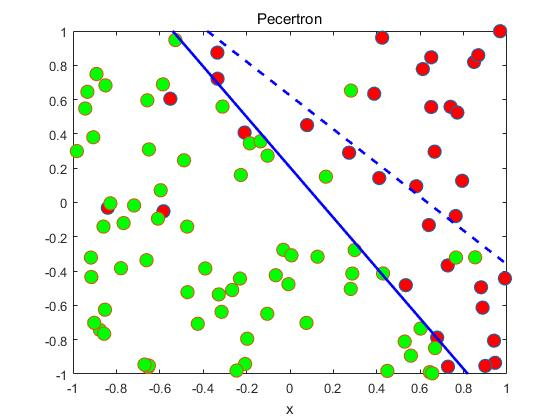
\includegraphics[height=2in]{./Perceptron_nonlinear.jpg}
\end{center}




\subsection{Linear Regression}

(i) the the trainning set is 100, trainning error rate is 0.0384, and the test error rate is 0.04809. The decision boundary is shown below.

\begin{center}
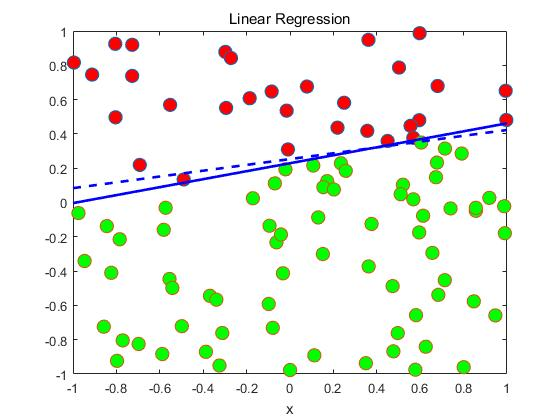
\includegraphics[height=2in]{./LinearReg_i.jpg}
\end{center}

(ii) When the dataset is not linearly separable, the trainning error rate is 0.1375, and the test error rate is 0.0620. The decision boundary is shown below.

\begin{center}
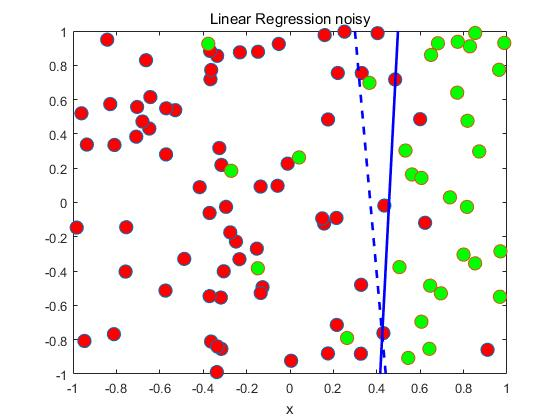
\includegraphics[height=2in]{./LinearReg_ii.jpg}
\end{center}

(iii) For the dataset \emph{poly\_train.mat}, the trainint error rate is 0.4900, the testing error rate is 0.5496.

(iv) After transforming the input data, the training error rate is 0.0500, the testing error rate is 0.0660.

\subsection{Logistic Regression}

I use following parameters in \emph{logistic.m}:

$learning\_rate = 0.02$ and 
$max\_iter = 5000$

(i) If the size of training set is 100, the trainning error rate is 0.0191, and the testing error rate is 0.0292. The decision boundary is shown below.

\begin{center}
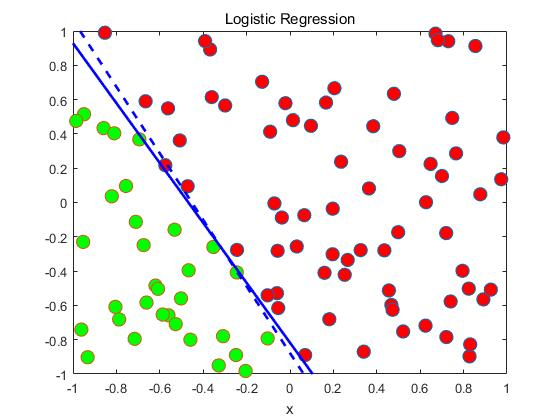
\includegraphics[height=2in]{./Logistic_i.jpg}
\end{center}

(ii) When the training data is not linearly separable, the training error rate is 0.1284, and the testing error rate is 0.0493. The decision boundary is shown below.

\begin{center}
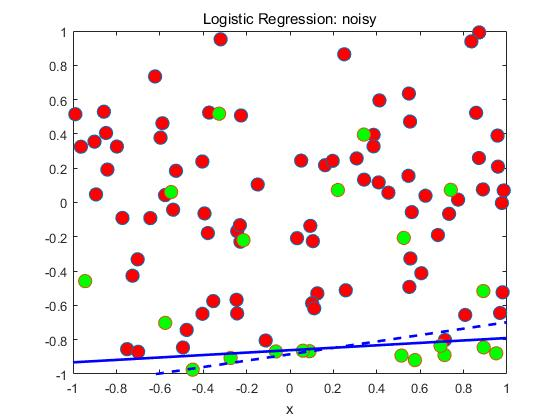
\includegraphics[height=2in]{./Logistic_ii.jpg}
\end{center}


\subsection{SVM}

(i) If the size of training set is 30, the training error rate is 0.00, and the tesing error rate is 0.0376. The decision boundary is shown below.

\begin{center}
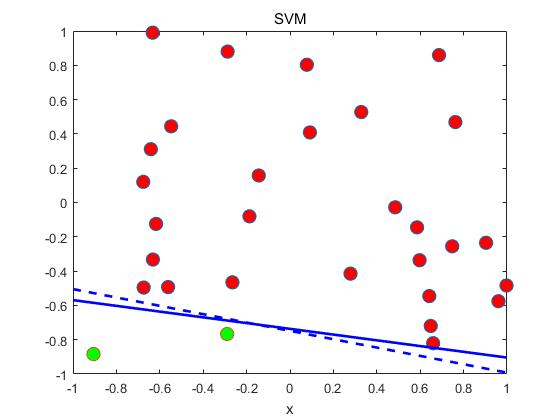
\includegraphics[height=2in]{./SVM_i.jpg}
\end{center}

(ii) If the size of training set is 100, the training error rate is 0.00, and the tesing error rate is 0.0111. The decision boundary is shown below.

\begin{center}
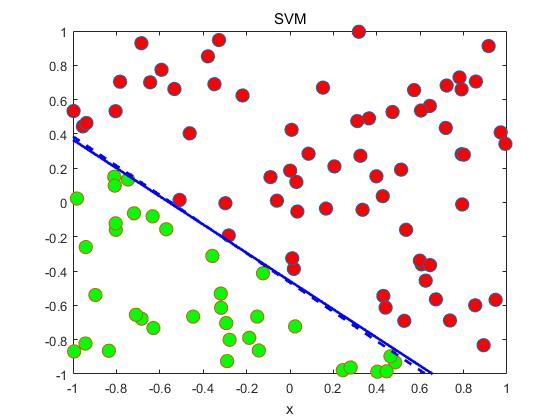
\includegraphics[height=2in]{./SVM_ii.jpg}
\end{center} 

(iii) For the cane nTrain = 100, the average number of support vectors is 2.8440

\end{document}
